\section{Big data}

Effectively leveraging big data requires the establishment of a comprehensive data management process that encompasses all stages of the data pipeline. 
This process includes data collection, ingestion, analysis, and the ultimate creation of value. 
Each stage is critical to transforming raw data into actionable insights that can drive decision-making and generate tangible benefits. 
The key components of this process are outlined below:
\begin{enumerate}
    \item \textit{Data collection}: gathering data from a wide range of sources is the foundation of any big data initiative. 
    \item \textit{Data analysis}: the collected data must be meticulously analyzed to uncover patterns, trends, and insights. 
        This analysis is tailored to the needs of various stakeholders.
        Analytical methods include descriptive analysis, which provides a snapshot of current data trends, and predictive analysis, which forecasts future developments.
    \item \textit{Value creation}: the final step in the data pipeline is the creation of value from the analyzed data. 
        This value can manifest in several ways.
\end{enumerate} 
Big data is becoming increasingly prevalent due to several key factors:
\begin{itemize}
    \item \textit{Declining storage costs}: as hard drives and storage technologies become more affordable, organizations can store vast amounts of data more economically, making it feasible to accumulate and analyze large datasets regularly.
    \item \textit{Ubiquitous data generation}: in today's digital age, we are all constant producers of data, whether through our interactions on social media, the use of smart devices, or routine activities online. 
        This continuous data generation contributes to the exponential growth of big data.
    \item \textit{Rapid data growth}: the volume of data is expanding at a rate that far outpaces the growth in IT spending. 
        This disparity drives the need for more efficient and scalable data management solutions to keep up with the increasing data demands across various industries.
\end{itemize}
Big data is characterized by several key attributes that distinguish it from traditional data management paradigms. 
These attributes include:
\begin{itemize}
    \item \textit{Volume}: refers to the immense scale of data generated and stored. 
        Big data encompasses vast quantities, ranging from terabytes to exabytes, made possible by increasingly affordable storage solutions.
    \item \textit{Variety}: describes the diverse forms in which data is available. 
        Big data includes structured data (such as databases), unstructured data (like text and emails), and multimedia content (including images, videos, and audio).
    \item \textit{Velocity}: represents the speed at which data is generated, processed, and analyzed. 
        Big data often involves real-time or near-real-time data streams, enabling rapid decision-making within fractions of a second.
    \item \textit{Veracity}: concerns the uncertainty and reliability of data. 
        Big data often includes information that may be imprecise, incomplete, or uncertain, requiring robust methods to manage and ensure data accuracy and predictability.
\end{itemize}   

\subsection{Data analysis}
As the amount of data continues to grow, our methods for solving data-related problems must also evolve. 
In the traditional approach, analysis was typically performed on a small subset of information due to limitations in data processing capabilities. 
However, with big data, we adopt an innovative approach that allows us to analyze all available information, providing a more comprehensive understanding and deeper insights.
\begin{figure}[H]
    \centering
    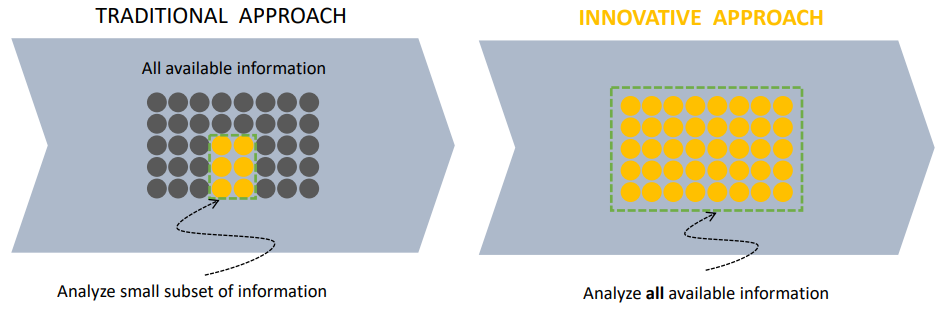
\includegraphics[width=0.75\linewidth]{images/in.png}
    \caption{More data analyzed}
\end{figure}
In the traditional approach, we typically start with a hypothesis and test it against a selected subset of data. 
This method is limited by the scope and size of the data sample.
In contrast, the innovative approach used in big data allows us to explore all available data, enabling the identification of correlations and patterns without pre-established hypotheses.
This data-driven exploration opens up new possibilities for discovering insights that might have been overlooked using traditional methods.
\begin{figure}[H]
    \centering
    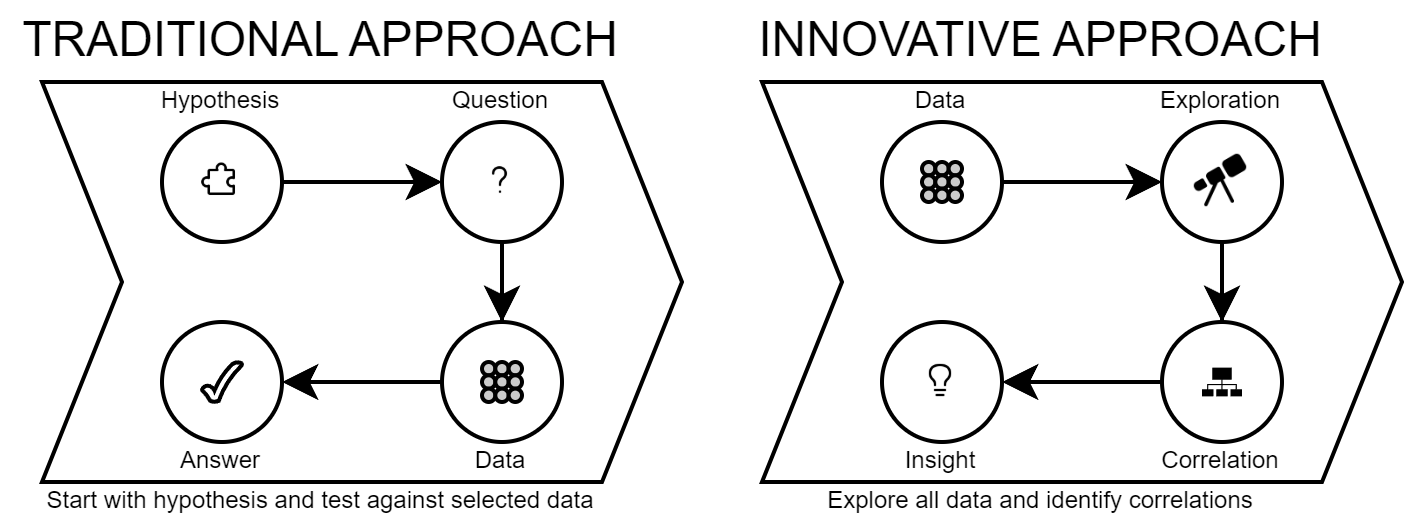
\includegraphics[width=0.75\linewidth]{images/in1.png}
    \caption{Data driven exploration}
\end{figure}
In the traditional approach, we meticulously cleanse data before any analysis, resulting in a small, well-organized dataset. 
In contrast, the innovative approach involves analyzing data in its raw form and cleansing it as necessary, allowing us to work with a larger volume of messy information.
\begin{figure}[H]
    \centering
    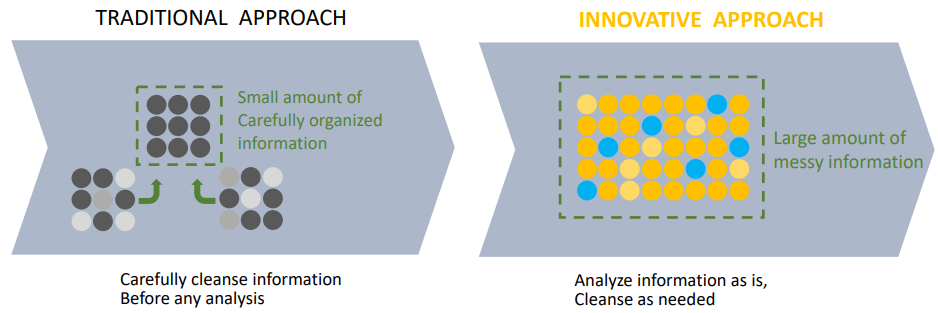
\includegraphics[width=0.75\linewidth]{images/in2.png}
    \caption{Less effort}
\end{figure}
In the traditional approach, data is analyzed only after it has been processed and stored in a warehouse or data mart. 
Meanwhile, the innovative approach focuses on analyzing data in motion, in real-time as it is generated.
\begin{figure}[H]
    \centering
    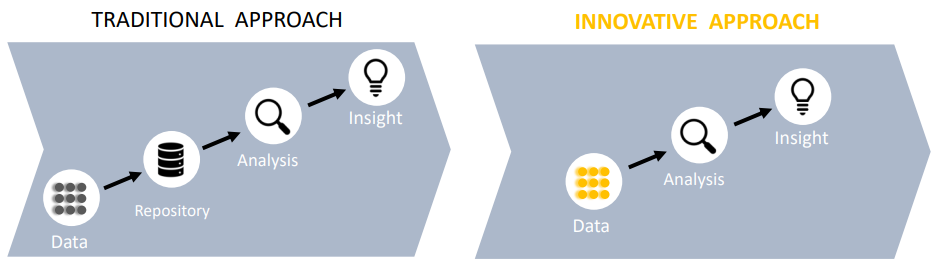
\includegraphics[width=0.75\linewidth]{images/in3.png}
    \caption{Streaming data}
\end{figure}